\subsection{Szövegformázás}

%53
\begin{frame}
  \begin{description}[m]
    \item[\texttt{text-align}] \hfill \\ Vízszintes igazítás: \texttt{left} (balra), \texttt{center} (középre), \texttt{right} (jobbra), \texttt{justify} (sorkizárt)
  \end{description}
  \begin{columns}[c]
    \column{0.6\textwidth}
      \begin{exampleblock}{\textattachfile{vizszintes.html}{vizszintes.html}}
        \tiny
        \lstinputlisting[style=HTML,linerange={7-10},numbers=left,firstnumber=7]{vizszintes.html}
        \lstinputlisting[style=HTML,linerange={15-16},numbers=left,firstnumber=15]{vizszintes.html}
      \end{exampleblock}
    \column{0.35\textwidth}
      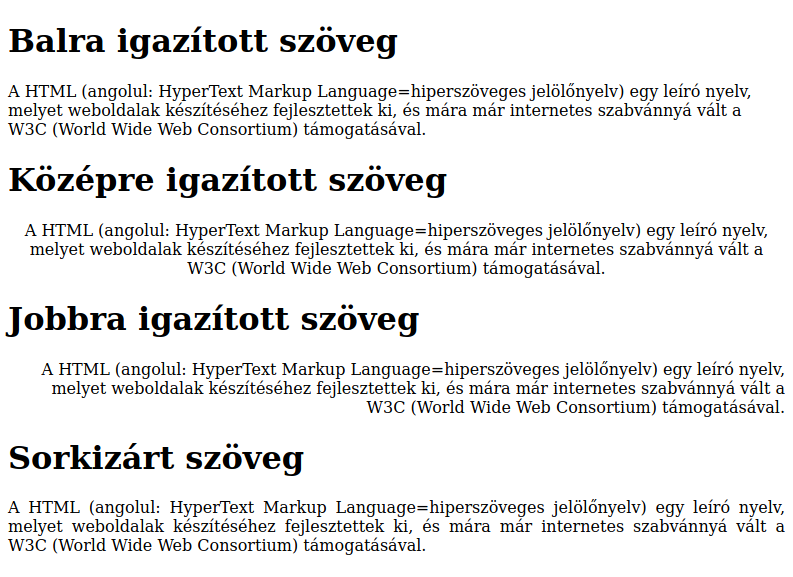
\includegraphics[width=\textwidth]{vizszintes.png}
  \end{columns}
\end{frame}

%54
\begin{frame}
  \texttt{hyphens}: elválasztások, hogy a szöveg tördelése még finomabb legyen
  \begin{description}[m]
    \item[\texttt{none}] \hfill \\ nincs elválasztás, alapértelmezés
    \item[\texttt{manual}] \hfill \\ elválasztás csak a kézzel előre megjelölt helyeken (\texttt{\&hyphen;}, \texttt{\&shy;})
    \item[\texttt{auto}] \hfill \\ automatikus elválasztás
  \end{description}
\end{frame}

%55
\begin{frame}
  \begin{exampleblock}{\textattachfile{elvalasztas.html}{elvalasztas.html}}
    \scriptsize
    \lstinputlisting[style=HTML,linerange={8-8},numbers=left,firstnumber=8]{elvalasztas.html}
    \lstinputlisting[style=HTML,linerange={12-13},numbers=left,firstnumber=12]{elvalasztas.html}
    \lstinputlisting[style=HTML,linerange={16-16},numbers=left,firstnumber=16]{elvalasztas.html}
  \end{exampleblock}
  \begin{center}
    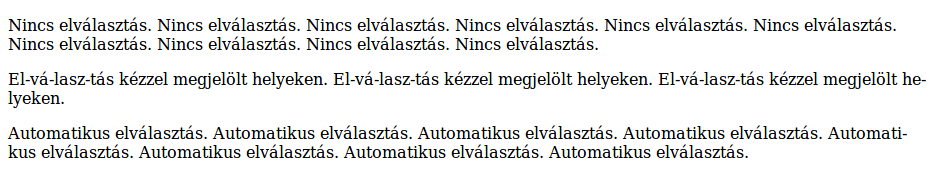
\includegraphics[width=\textwidth]{elvalasztas.png}
  \end{center}
\end{frame}

%56
\begin{frame}
  \texttt{vertical-align}: tetszőleges elem függőleges igazítása
  \begin{description}[m]
    \item[\texttt{baseline}] \hfill \\ szülő szövegének alapvonalához
    \item[\emph{távolság}] \hfill \\ tetszőleges mértékű süllyesztéshez/emeléshez, negatív érték is elfogadott
    \item[\texttt{\%}] \hfill \\ sormagasság \%-ában megadott emelés/süllyesztés, negatív érték is elfogadott
    \item[\texttt{sub}] \hfill \\ szülő alsó indexéhez
    \item[\texttt{super}] \hfill \\ szülő felső indexéhez
  \end{description}
\end{frame}

%57
\begin{frame}
  \begin{description}[m]
    \item[\texttt{top}] \hfill \\ sor legmagasabb eleméhez
    \item[\texttt{text-top}] \hfill \\ szülő elem szövegének tetejéhez
    \item[\texttt{middle}] \hfill \\ szülő közepéhez
    \item[\texttt{bottom}] \hfill \\  sor legalsó eleméhez
    \item[\texttt{text-bottom}] \hfill \\ szülő szövegének aljához
  \end{description}
\end{frame}

%58
\begin{frame}
  \begin{columns}[c]
    \column{0.55\textwidth}
      \begin{exampleblock}{\textattachfile{fuggoleges.html}{fuggoleges.html}}
        \tiny
        \lstinputlisting[style=HTML,linerange={7-9},numbers=left,firstnumber=7]{fuggoleges.html}
        \lstinputlisting[style=HTML,linerange={13-15},numbers=left,firstnumber=13]{fuggoleges.html}
      \end{exampleblock}
    \column{0.4\textwidth}
      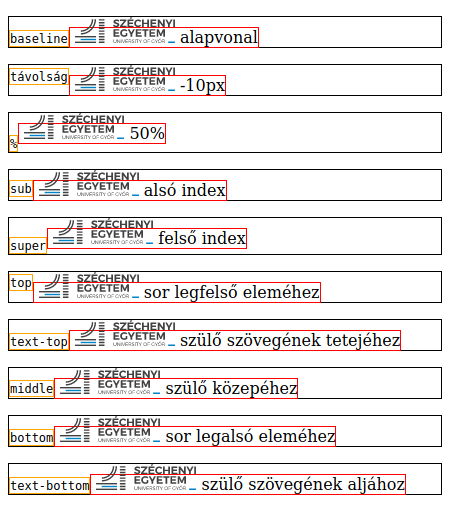
\includegraphics[width=\textwidth]{fuggoleges.png}
  \end{columns}
\end{frame}

%59
\begin{frame}
  \begin{description}[m]
    \item[\texttt{text-indent}] \hfill \\ Első sor behúzása: \emph{távolság} (a bekezdés bal szélétől számított behúzás), \texttt{\%} (szülő elem szélességének százalékában adott behúzás)
  \end{description}
  \begin{columns}[c]
    \column{0.6\textwidth}
      \begin{exampleblock}{\textattachfile{behuzas.html}{behuzas.html}}
        \tiny
        \lstinputlisting[style=HTML,linerange={7-10},numbers=left,firstnumber=7]{behuzas.html}
        \lstinputlisting[style=HTML,linerange={14-16},numbers=left,firstnumber=14]{behuzas.html}
      \end{exampleblock}
    \column{0.35\textwidth}
      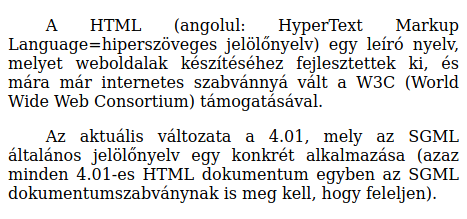
\includegraphics[width=\textwidth]{behuzas.png}
  \end{columns}
\end{frame}

%60
\begin{frame}
  \texttt{white-space}: fehér karakterek értelmezése
  \begin{description}[m]
    \item[\texttt{normal}] \hfill \\ szomszédos fehér karaktereket összevonja, alapértelmezés
    \item[\texttt{nowrap}] \hfill \\ nem tördeli a hosszú sorokat, de a szomszédos fehér karaktereket összevonja
    \item[\texttt{pre}] \hfill \\ utánozza a \texttt{<pre>} HTML elem működését, minden fehér karaktert megőriz
    \item[\texttt{pre-line}] \hfill \\ szomszédos fehér karaktereket összevonja, de tördeli a sorokat, ha szükséges
    \item[\texttt{pre-wrap}] \hfill \\ minden fehér karaktert megőriz, és tördel, ha szükséges
  \end{description}
\end{frame}

%61
\begin{frame}
  Nem választ magától \texttt{monospace} karakterkészletet!
  \begin{columns}[c]
    \column{0.6\textwidth}
      \begin{exampleblock}{\textattachfile{fahrcels2.html}{fahrcels2.html}}
        \footnotesize
        \lstinputlisting[style=HTML,linerange={7-10},numbers=left,firstnumber=7]{fahrcels2.html}
        \lstinputlisting[style=HTML,linerange={14-16},numbers=left,firstnumber=14]{fahrcels2.html}
      \end{exampleblock}
    \column{0.35\textwidth}
      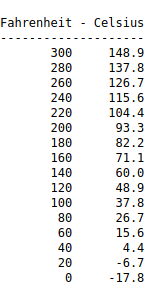
\includegraphics[width=0.7\textwidth]{fahrcels2.png}
  \end{columns}
\end{frame}

%62
\begin{frame}
  \texttt{letter-spacing}: betűk közötti távolság
  \begin{description}[m]
    \item[\texttt{normal}] \hfill \\ szokásos távolság, alapértelmezés
    \item[\emph{távolság}] \hfill \\ betűk közötti távolság, negatív érték is elfogadott
  \end{description}
  \vfill
  \texttt{word-spacing}: szavak közötti távolság
  \begin{description}[m]
    \item[\texttt{normal}] \hfill \\ szokásos távolság (betűmagasság negyede), alapértelmezés
    \item[\emph{távolság}] \hfill \\ szavak közötti távolság, negatív érték is elfogadott
  \end{description}
\end{frame}

%63
\begin{frame}
  \begin{exampleblock}{\textattachfile{tavolsag.html}{tavolsag.html}}
    \footnotesize
    \lstinputlisting[style=HTML,linerange={7-11},numbers=left,firstnumber=7]{tavolsag.html}
    \lstinputlisting[style=HTML,linerange={15-16},numbers=left,firstnumber=15]{tavolsag.html}
  \end{exampleblock}
  \begin{center}
    
\includegraphics[width=0.8\textwidth]{tavolsag.png}
  \end{center}
\end{frame}

%64
\begin{frame}
  \texttt{text-transform}: szöveg átalakítása
  \begin{description}[m]
    \item[\texttt{normal}] \hfill \\ nincs átalakítás, alapértelmezés
    \item[\texttt{capitalize}] \hfill \\ minden kezdőbetűt nagybetűvel nyomtat
    \item[\texttt{uppercase}] \hfill \\ csupa nagybetűvel nyomtat
    \item[\texttt{lowercase}] \hfill \\ csupa kisbetűvel nyomtat
  \end{description}
\end{frame}

%65
\begin{frame}
  \begin{exampleblock}{\textattachfile{nagybetu.html}{nagybetu.html}}
    \scriptsize
    \lstinputlisting[style=HTML,linerange={7-9},numbers=left,firstnumber=7]{nagybetu.html}
    \lstinputlisting[style=HTML,linerange={13-14},numbers=left,firstnumber=13]{nagybetu.html}
  \end{exampleblock}
  \begin{center}
    
\includegraphics[scale=0.5]{nagybetu.png}
  \end{center}
\end{frame}

%66
\begin{frame}
  \texttt{text-decoration-line}: vonal húzása a szöveggel párhuzamosan
  \begin{description}[m]
    \item[\texttt{none}] \hfill \\ nincs vonalazás, alapértelmezés. Pl. hivatkozások aláhúzásának eltávolításához használható.
    \item[\texttt{underline}] \hfill \\ aláhúzza a szöveget; \kiemel{félrevezetheti az olvasót}, ha nem csak a hivatkozások jelennek meg aláhúzással!
    \item[\texttt{overline}] \hfill \\ a szöveg fölött húz vonalat
    \item[\texttt{line-through}] \hfill \\ áthúzza a szöveget
  \end{description}
\end{frame}

%67
\begin{frame}
  \texttt{text-decoration-style}: a vonal stílusa
  \begin{description}[m]
    \item[\texttt{solid}] \hfill \\ folytonos vonal
    \item[\texttt{double}] \hfill \\ dupla vonal
    \item[\texttt{dotted}] \hfill \\ pontvonal
    \item[\texttt{dashed}] \hfill \\ szaggatott vonal
    \item[\texttt{wavy}] \hfill \\ hullámos vonal
  \end{description}
\end{frame}

%68
\begin{frame}
  \texttt{text-decoration-color}: a vonal színe
  \begin{description}[m]
    \item[\emph{szín}] \hfill \\ tetszőleges CSS színmegadási móddal
  \end{description}
  \vfill
  Rövidítés:
  \begin{description}[m]
    \item[\texttt{text-decoration:}]
    \item[\qquad\texttt{text-decoration-line text-decoration-color text-decoration-style}] \hfill \\ Akár többféle vonal is megadható, tetszőleges rész elhagyható, sorrend tetszőleges
  \end{description}
\end{frame}

%69
\begin{frame}
  \begin{exampleblock}{\textattachfile{dekoracio.html}{dekoracio.html}}
    \footnotesize
    \lstinputlisting[style=HTML,linerange={7-11},numbers=left,firstnumber=7]{dekoracio.html}
    \lstinputlisting[style=HTML,linerange={15-17},numbers=left,firstnumber=15]{dekoracio.html}
  \end{exampleblock}
  \begin{center}
    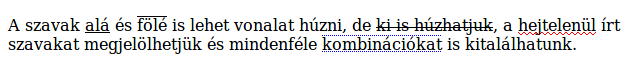
\includegraphics[width=\textwidth]{dekoracio.png}
  \end{center}
\end{frame}

%70
\begin{frame}
  \texttt{text-shadow}: szöveg árnyéka
  \begin{description}[m]
    \item[\texttt{h-shadow v-shadow blur-radius color}] \hfill \\ vízszintes eltolás, függőleges eltolás, elmosás mértéke, szín. \\ Az elmosás mértéke elhagyható, a többi kötelező. Az eltolásoknál negatív értékek megengedettek. Vesszővel elválasztva több árnyék is megadható egyszerre.
    \item[\texttt{none}] nincs árnyék, alapértelmezés
  \end{description}
\end{frame}

%71
\begin{frame}
  \begin{columns}[c]
    \column{0.7\textwidth}
      \begin{exampleblock}{\textattachfile{arnyek.html}{arnyek.html}}
        \scriptsize
        \lstinputlisting[style=HTML,linerange={7-12},numbers=left,firstnumber=7]{arnyek.html}
        \lstinputlisting[style=HTML,linerange={16-18},numbers=left,firstnumber=16]{arnyek.html}
      \end{exampleblock}
    \column{0.25\textwidth}
      
\includegraphics[width=\textwidth]{arnyek.png}
  \end{columns}
\end{frame}

%72
\begin{frame}
  \texttt{line-height}: sormagasság
  \begin{description}[m]
    \item[\texttt{normal}] \hfill \\ betűméretből következő sormagasság, alapértelmezett
    \item[\emph{szám}] \hfill \\ az aktuális betűméretet ezzel szorozva kapja meg a sormagasságot
    \item[\emph{távolság}] \hfill \\ rögzített sormagasság, CSS mértékegységben
    \item[\texttt{\%}] \hfill \\ az aktuális betűméret \%-a
  \end{description}
\end{frame}

%73
\begin{frame}
  \begin{columns}[c]
    \column{0.65\textwidth}
      \begin{exampleblock}{\textattachfile{sormagassag.html}{sormagassag.html}}
        \scriptsize
        \lstinputlisting[style=HTML,linerange={7-9},numbers=left,firstnumber=7]{sormagassag.html}
        \lstinputlisting[style=HTML,linerange={13-15},numbers=left,firstnumber=13]{sormagassag.html}
      \end{exampleblock}
    \column{0.3\textwidth}
      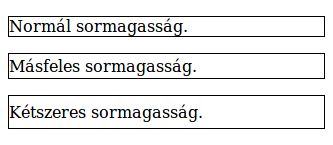
\includegraphics[width=\textwidth]{sormagassag.png}
  \end{columns}
\end{frame}

%74
\begin{frame}
  Többféle írásirány támogatott egyazon oldalon
  \begin{columns}[c]
    \column{0.65\textwidth}
      \begin{exampleblock}{\textattachfile{irasirany.html}{irasirany.html}}
        \footnotesize
        \lstinputlisting[style=HTML,linerange={7-10},numbers=left,firstnumber=7]{irasirany.html}
        \lstinputlisting[style=HTML,linerange={14-15},numbers=left,firstnumber=14]{irasirany.html}
      \end{exampleblock}
    \column{0.3\textwidth}
      
\includegraphics[width=\textwidth]{irasirany.png}
  \end{columns}  
\end{frame}

%75
\begin{frame}
  \begin{columns}[c]
    \column{0.5\textwidth}
      \footnotesize
      Készítse el az ábrán látható weboldalt!
      \begin{itemize}
        \item Induljon ki a \textattachfile{szoveg.txt}{szoveg.txt} fájlból!
        \item A címsor betűi között hagyjon 5-5 képpontnyi helyet,
        \item írja csupa nagybetűvel, és
        \item jelenítsen meg alatta 3-3 képpontnyival jobbra és lefelé eltolt árnyékot, mely kék színű, és elmosásának sugara 10 képpont!
        \item A bekezdés legyen sorkizárt igazítású, 
        \item a sormagasság másfélszeres,
        \item az első sor behúzása 20 képpontnyi,
        \item és automatikusan elválasztott!
        \item Az emberek neveit emelje ki zöld színű, dupla aláhúzással!
      \end{itemize}
    \column{0.45\textwidth}
      \begin{exampleblock}{\textattachfile{szoveg.html}{szoveg.html}}
        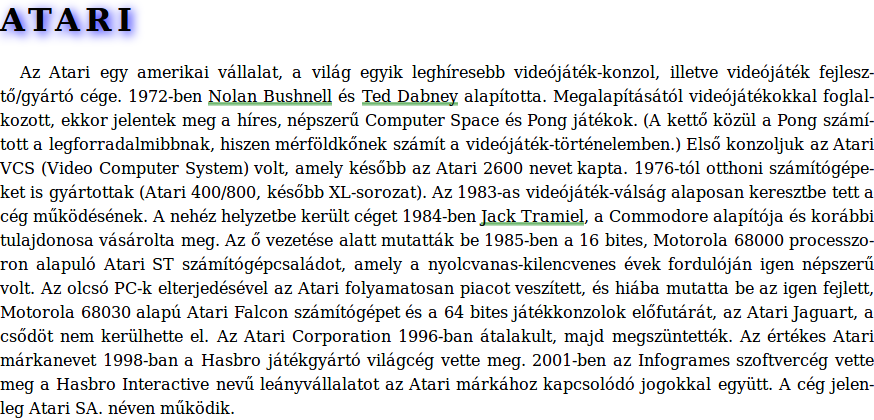
\includegraphics[width=\textwidth]{szoveg.png}
      \end{exampleblock}
  \end{columns}
\end{frame}
